\documentclass[CS4402-Notes.tex]{subfiles}
\begin{document}

\section{Introduction}

\subsection{Constraint satisfaction problem}
The constraint satisfaction problem is a general way in which decision-making problems can be represented and solved. It is defined as follows:
\textbf{Given}
\begin{itemize}
\item A set of \textbf{decision variables} - A decision variable corresponds to a choice that must be made in solving a problem. For example in university timetabling, various things have to be decided, such as time for each lecture and venue for each lecture
\item For each decision variable, a \textbf{domain} of potential values - Values in the domain of a decision variable correspond to the options for a particular choice. When a decision variable is assigned a single value from its domain, it is equivalent to the choice associated with that variable being made. 
\item A set of \textbf{constraints} on the decision variables. The \textbf{scope} of a constraint is a subset of the decision variables a constraint involves. Out of all possible combinations of assignments to the variables in its scope, a constraint specifies which assignments are allowed (satisfy the constraint) and which are disallowed (violet the constraint). 
\end{itemize}
Find an \textbf{assignment} of values to variables such that all constraints are satisfied.
\n
There are two main phases to solving problems with constraints: \textbf{Modelling} and \textbf{Solving}.
\subsubsection{Constraint modelling}
A constraint model maps the features of a given problem onto the features of a constraint satisfaction problem. In other words, the input problem must be modelled in a way that is represented with decisions variables, domains and constraints. 
\begin{figure}[H]
\centering
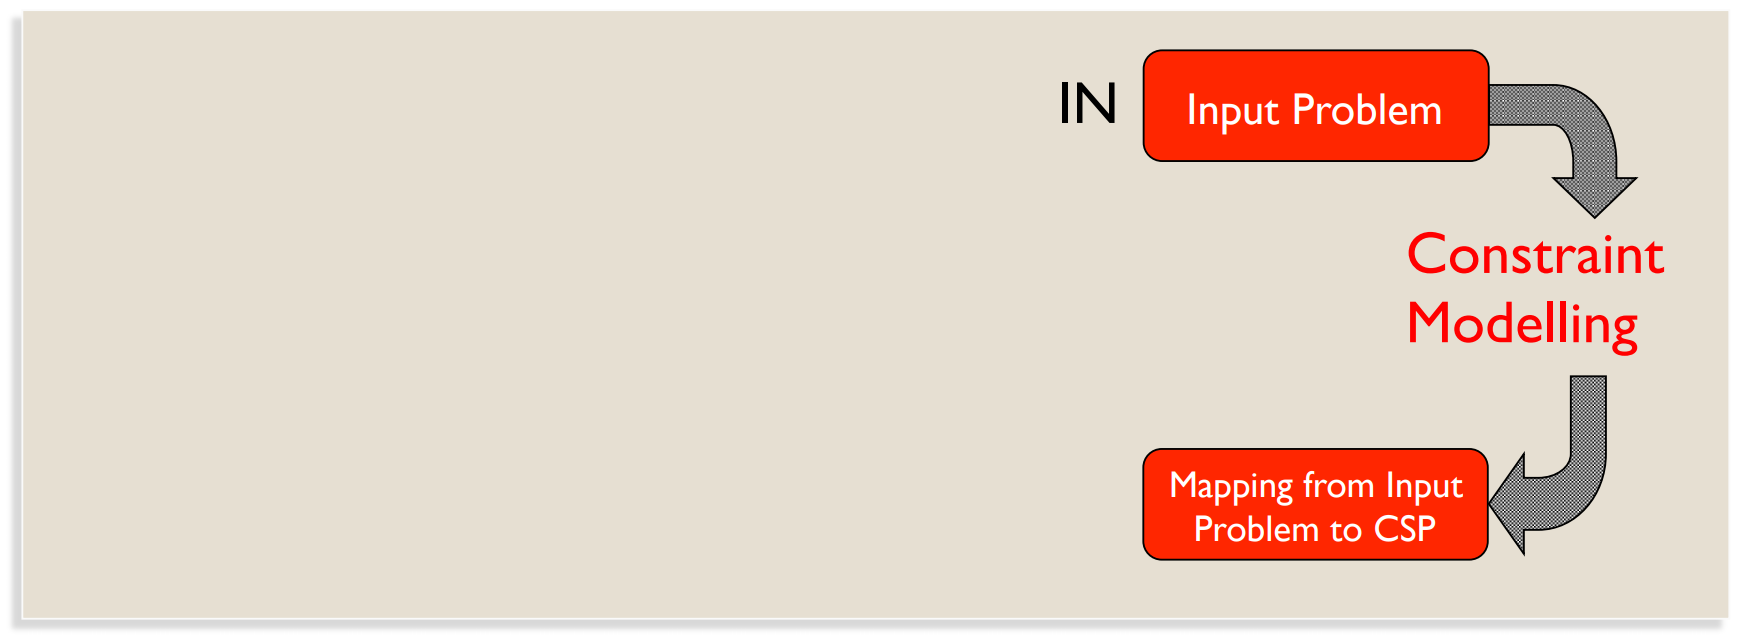
\includegraphics[width=1\textwidth, keepaspectratio]{imgs/constraint-modelling.png}
\caption{Constraint modelling is the first step in solving constraint problems.}
\end{figure}

\subsubsection{Constraint solving}
\begin{figure}[H]
\centering
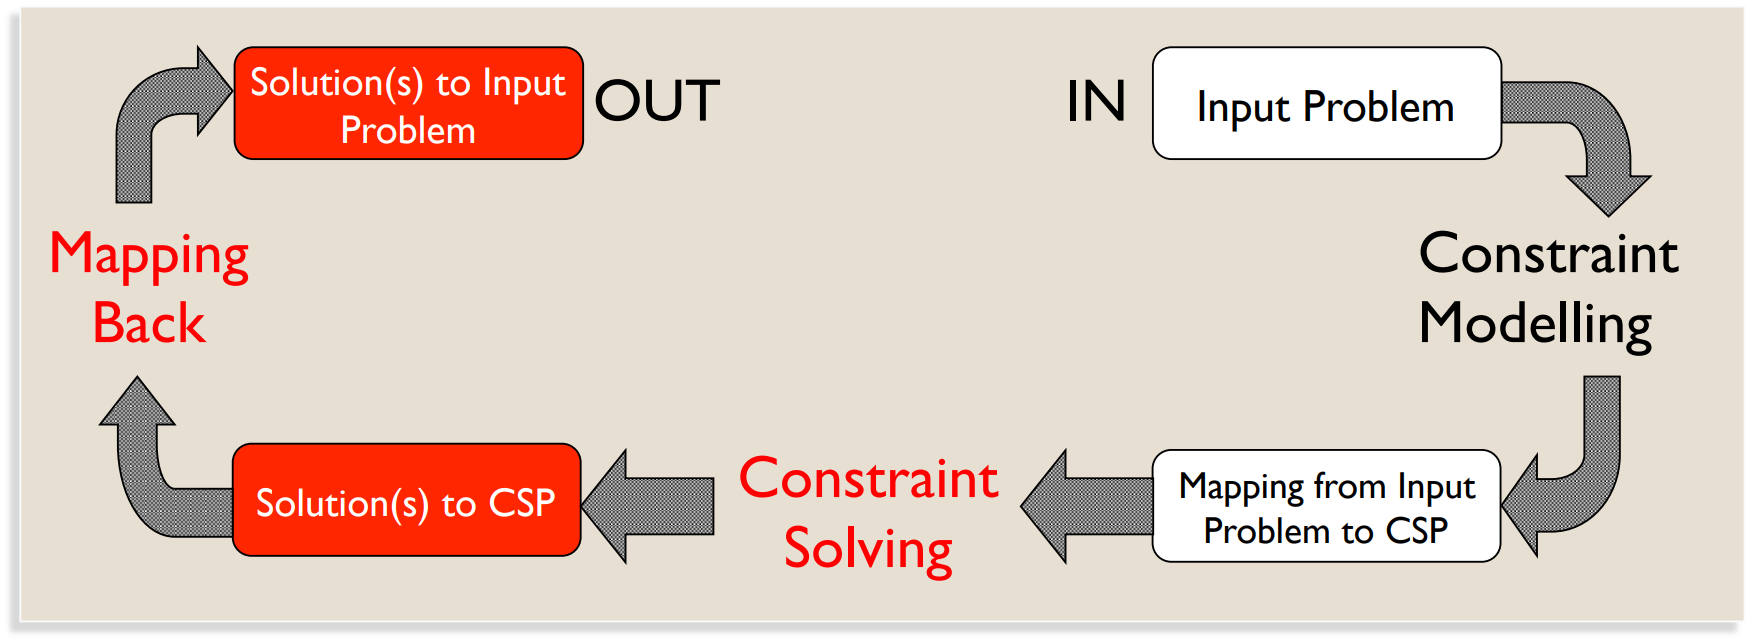
\includegraphics[width=1\textwidth, keepaspectratio]{imgs/constraint-solving.png}
\caption{Full pipeline of constraint solving.}
\end{figure}
\noindent
The modelled CSP is used as input to a constraint solver, which produces one or more solutions. To find solutions, a solver combines \textbf{search} and \textbf{deduction}. 
\begin{enumerate}
\item A systematic search through the space of partial assignments makes guesses about variable assignments. The assignments are done incrementally to a subset of the variables and the solver must backtrack if the current assignments cannot lead to a solution.
\item Constraint propagation is the way to make deductions based on constraints and current domains. This is usually recorded as reductions in domains so that when a variable has a single value left in its domain, that is part of the solution. 
\end{enumerate} 

\subsection{Constraint optimisation problem}
\begin{equation}
\text{COP} = \text{CSP} + \text{an objective function}
\end{equation}
The constraint optimisation problem adds an \textbf{objective function} to a normal CSP. The goal is then to maximise or minimise the objective function. The goal is then to find a solution where all constraints are satisfied \textit{and} the objective is optimised. Examples of these problems include minimising time taken in scheduling problems, or maximising profit. This gives four components to the constraint problem.
\begin{enumerate}
\item \textbf{Given} parameters
\item \textbf{Find} decision variables
\item \textbf{Such that} constraints
\item \textbf{Min/Maximising} objective
\end{enumerate}

\subsection{Problem classes}
A problem class describes a family of problems, related by a common set of \textbf{parameters}. Examples of a problem class is the n-queens problem class, or sudoku problem class. The parameters are the same as each problem instance in the class has the same rules. 
\n
It is important to note that constraint solvers solver problem \textbf{instances}. An instance is specified by instantiating the parameters of a problem class to particular values. In the sample of sudoku, a sudoku problem instance is the instantiation of the filled in hints given on the cells. Further, an individual CSP/COP represents a problem instance. 

\subsection{Constraint representation}
\subsubsection{Table constraint}
The table constraint is the most basic constraint available. It consists of listing the satisfying combination of assignments for all constraints and is known as the \textbf{extensional} representation. This is the most basic constraint as any constraint can be modelled in a table.
\n
For example given two variables
\begin{align*}
X\ \text{with domain}\ {1,2,3} \\
Y\ \text{with domain}\ {1,2}
\end{align*}
and the constraint $X > Y$, the table constraint would look as follows:
\begin{table}[H]
\centering
\begin{tabular}{| c |}
\hline
\textbf{Table(X, Y)} \\
\hline
$\langle 2, 1 \rangle$ \\
\hline
$\langle 3, 1 \rangle$ \\
\hline
$\langle 3, 2 \rangle$ \\
\hline
\end{tabular}
\end{table}
The issue with this basic constraint is that is can become both cumbersome and not practical. In an example of sudoku, where an AllDifferent constraint has to be imposed on 9 variable, the table would build to be $9!$ tuples large. The space to store the table tuples is not the only issue, as having to search through all the tuples would also take a significant amount of time. Because of this issue of combinatorial explosion, \textbf{intensional} representations were designed.

\subsubsection{Intensional constraints}
Rather than explicitly list all satisfying variable assignments, constraint solvers typically use intensional constraints to represent constraints like AllDifferent. This is done by the constraint solver by providing a library of commonly-occurring constraints that can be specified much more concisely. 
\n
However sometimes, the table (extensional) constraints must be used because it is the only sensible option, especially in examples where the constraint does not have an obvious algorithmic representation. This typically happens when the variables or domains are not numeric or easily represented as computing terms. 

\subsection{Constraint languages}
Constraint programmers often do not want to work directly with CSP/COPs as they can be both large and too low-level to work with. Instead, the CSP/COPs are written as constraint programs (models) in constraint languages. The program/model is essentially a recipe to follow that reproduces a CSP/COP. 
\n
In a constraint language, decision variables and their domains must be declared. This is often done with arrays of variables, which allows for iteration to model problem classes. Further, constraint models written in constraint languages specify the problem \textit{class} not the problem instance. The problem instances can be provided later as an instantiation of the parameters that the model specifies. Other common features in constraint languages include:
\begin{itemize}
\item Extensional constraints
\item Equality, disequality, inequality
\item Operators to build constraint expressions, for example +, -, AND, OR etc. These constraint expressions are then represented intensionally. 
\end{itemize}
The model written in constraint languages can be parameterised to represent a problem class. This is done by giving values for the parameters to obtain an instance which corresponds directly to a CSP/COP. The CSP/COP can then be passed to a constraint solver to get the solution to that instance.

\subsection{Crystal maze example}
\begin{figure}[H]
\centering
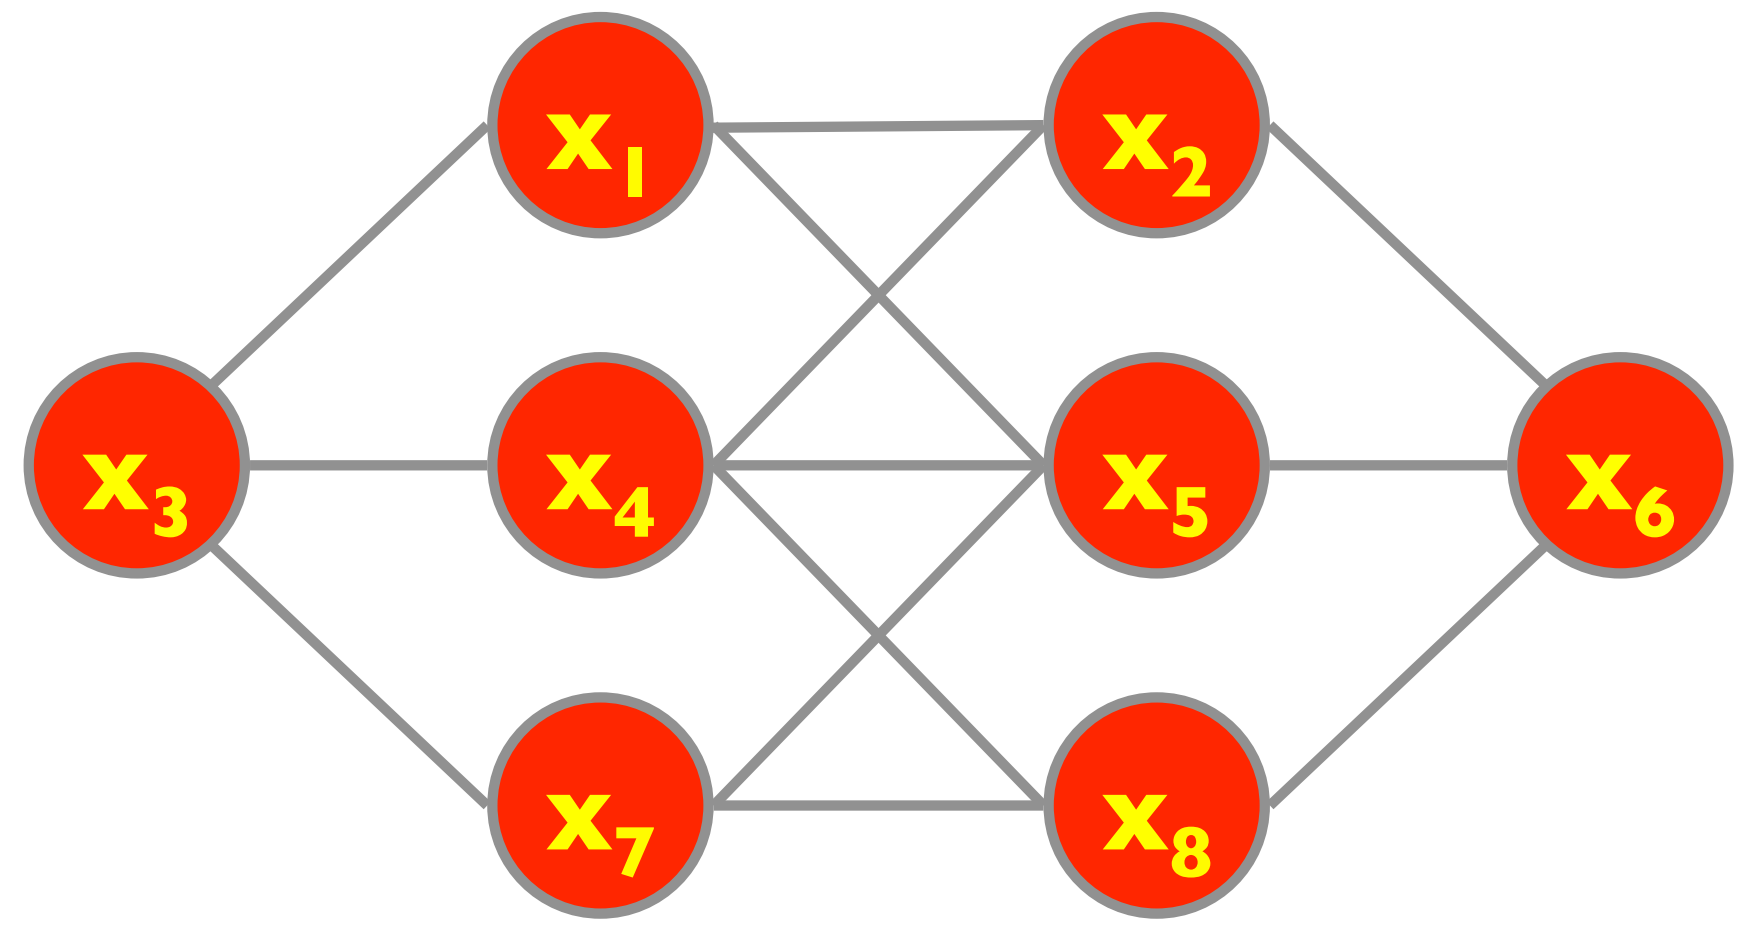
\includegraphics[width=0.75\textwidth, keepaspectratio]{imgs/crystal-maze.png}
\caption{The crystal maze puzzle.}
\end{figure}
\noindent
In the crystal maze puzzle, we must find $x_{1} ... x_{8}$ with each domain $\{1,2,3,4,5,6,7,8\}$ such that no adjacent nodes have adjacent values. For example, in the simple case of Constraint($x_{1}$, $x_{2}$), the table constraint would look as follows:
\begin{table}[H]
\centering
\begin{tabular}{| c |}
\hline
\textbf{Table($x_{1}, x_{2}$)} \\
\hline
$\langle 1, 1 \rangle$ \\
\hline
$\langle 1, 3 \rangle$ \\
\hline
$\langle 1, 4 \rangle$ \\
\hline
$...$ \\
\hline
$\langle 2, 2 \rangle$ \\
\hline
$\langle 2, 4 \rangle$ \\
\hline
$...$ \\
\hline
$\langle 8, 8 \rangle$ \\
\hline
\end{tabular}
\caption{50 possible combinations for each variable pairing that is connected.}
\end{table}
The table initially is populated with 64 possible constraints for all values in the domain of $x_{1}$ and $x_{2}$. However, the constraint that says all connected variables cannot be assigned consecutive numbers removes some of the value assignments. The same constraint can be expressed in an intensional representation with the following equation:
\begin{equation}
| x_{1} - x_{2} | \geq 1
\end{equation}
This works as it states that the values of $x_{1}$ and $x_{2}$ must have an absolute difference greater than 1. To be able to use the intensional representation, the constraint solver has to support the absolute value operator, subtraction operator and greater than constraint. 
\end{document}
